\chapter{Results}

\section{Model Diagnostics}
To perform inference, 120,000 (15,000 burn-in) draws of the unknown parameters from the posterior distribution were obtained using the adaptive Markov Chain Monte Carlo algorithm described in Chapter 3. Figure \ref{diagnostics} shows trace and autocorrelation plots for randomly selected marginal posteriors of $\beta$ and $\phi$ parameters, as well as the marginal posteriors for both $s$ and $\tau$. 
\begin{figure}[bt]
\centering
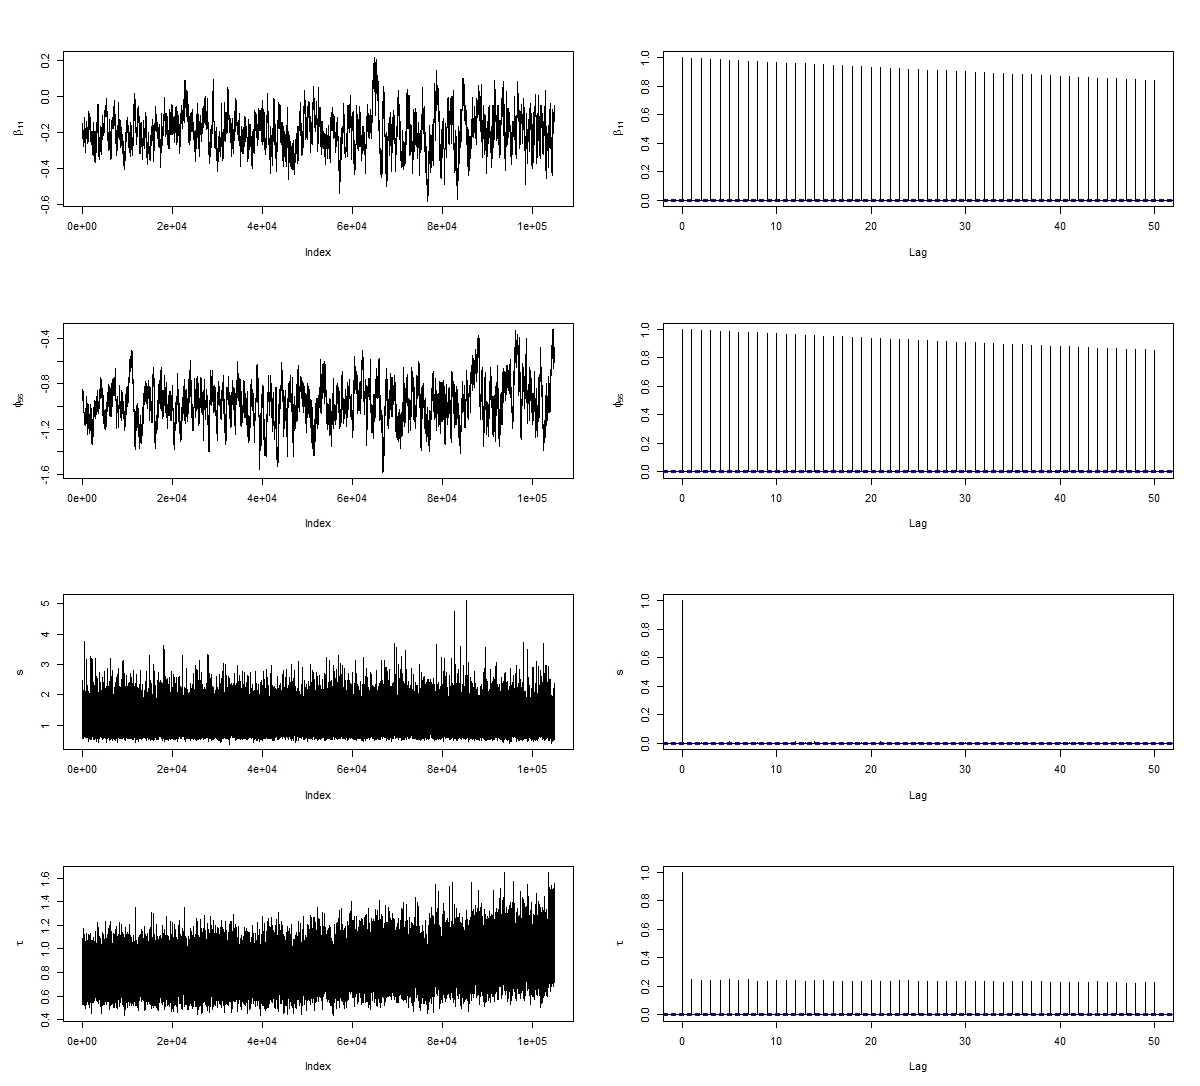
\includegraphics[width=.70\textwidth]{diagnostics.jpeg}
\caption{Trace and autocorrelation plots to assess convergence}
\label{diagnostics}
\end{figure}

Marginal distributions for nearly all $\beta$ and $\phi$ parameters have very high autocorrelation that can be seen in Figure \ref{diagnostics}. Despite the high autocorrelation, the trace plots show that the MCMC has sufficiently explored the parameter space. The trace and autocorrelation plots for $s$ and $\tau$ indicate adequate convergence. We further verify convergence of the MCMC draws using Monte Carlo (MC) standard errors \citep{jones06}. All of the MC standard errors for the $\beta$'s were less than .01 except for the intercept ($\beta_0$) which has a standard error of .014.   Likewise all of the MC standard errors for the $\phi$ parameters, except thirteen, were smaller than .01. However, the largest MC standard was .011 suggesting sufficiently high precision in the associated posterior summaries.

To verify that the fitted model explains the data well, Figure \ref{predictive} shows 95\% predictive intervals for each of the 207 road segments on I-35. Of the 207 intervals, 197 contain the observed value ($\approx 95\%$ coverage) suggesting that the model accurately captures the variation seen in the data.  Likewise, for I-35E, the predictive intervals have 97\% coverage also suggesting adequate model fit for I-35E.
\begin{figure}[h]
\centering
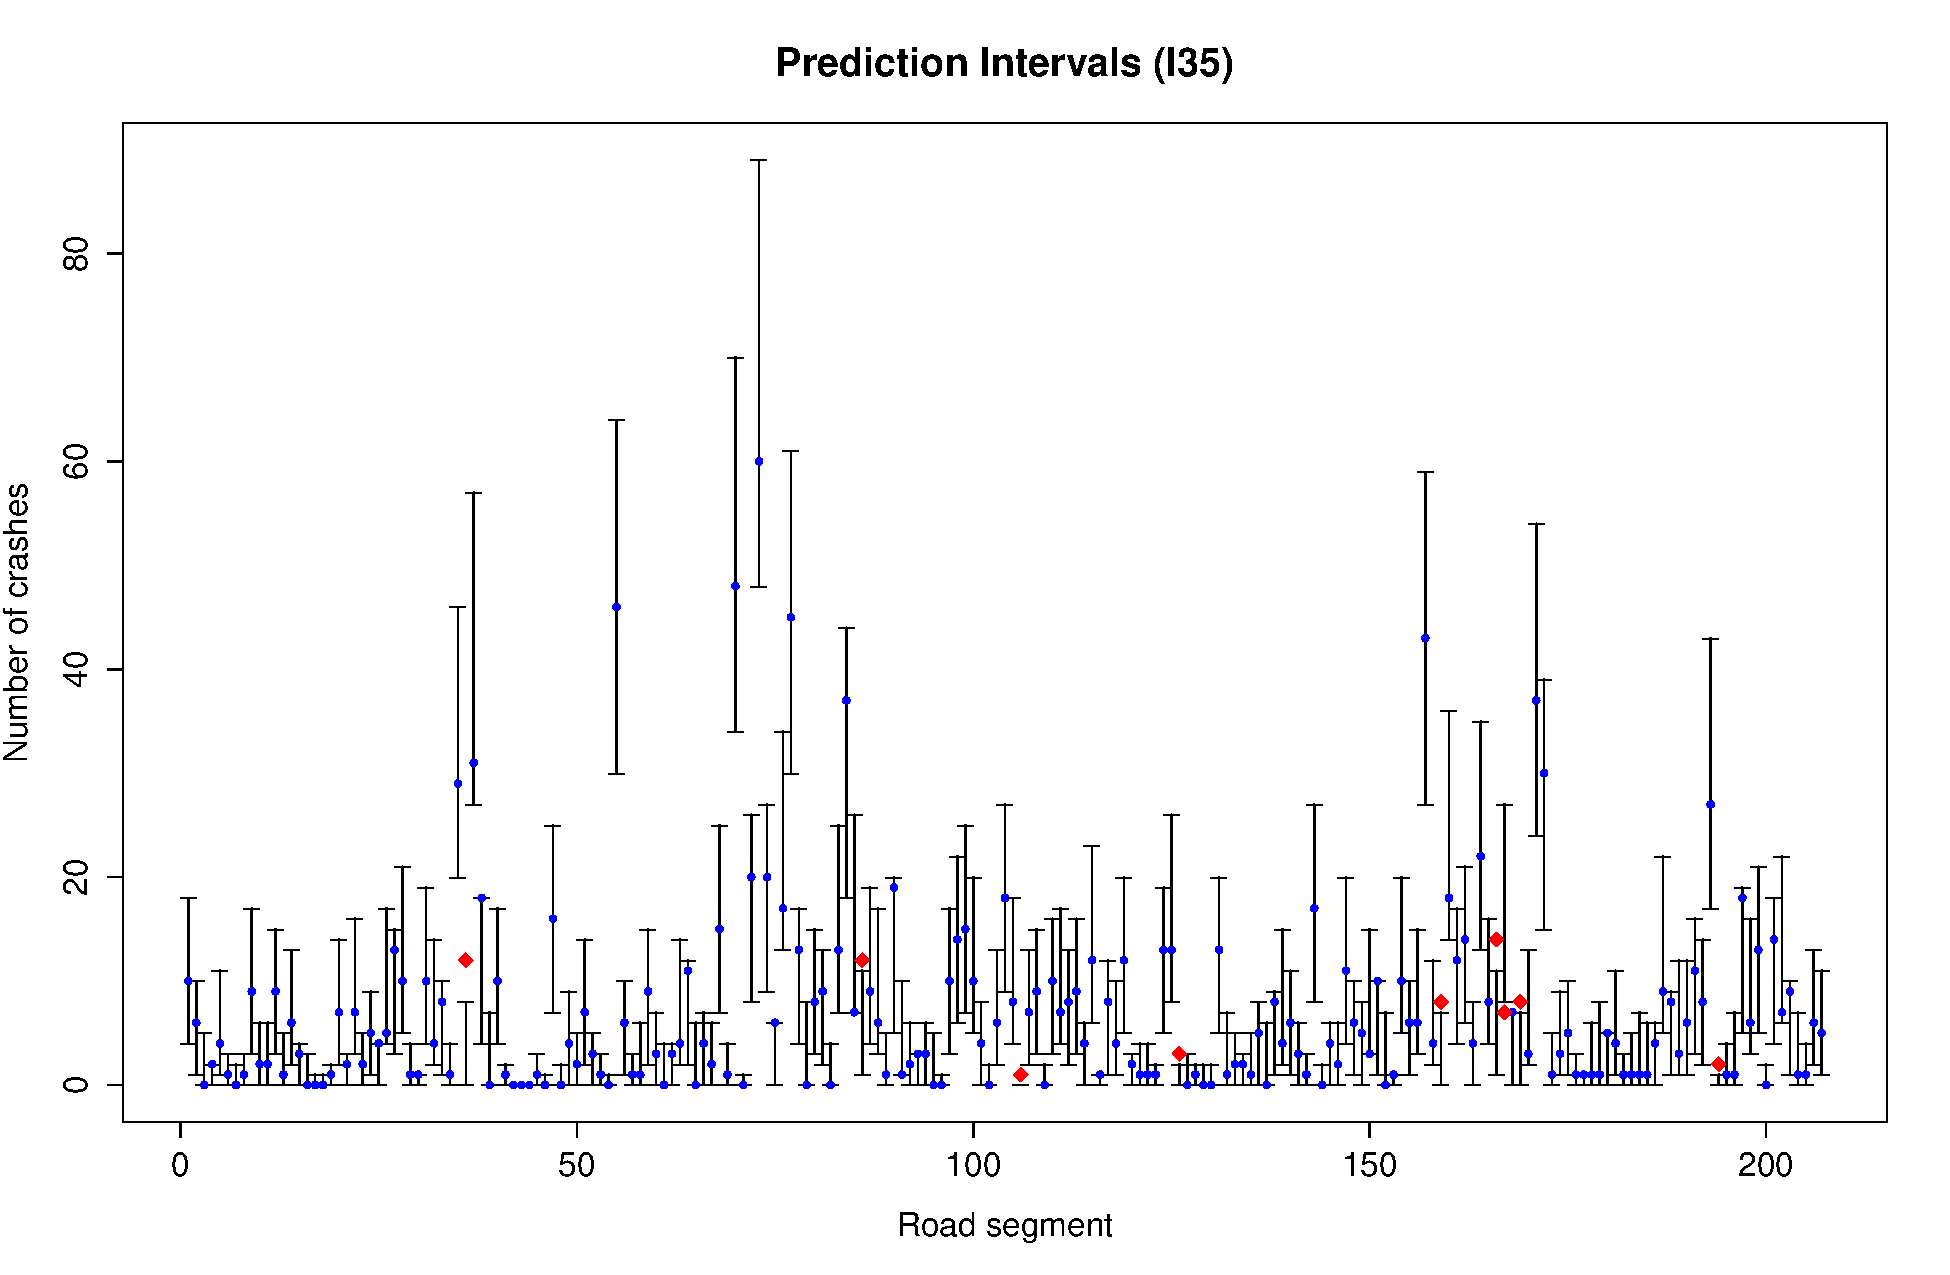
\includegraphics[width=.9\textwidth]{predictive.pdf}
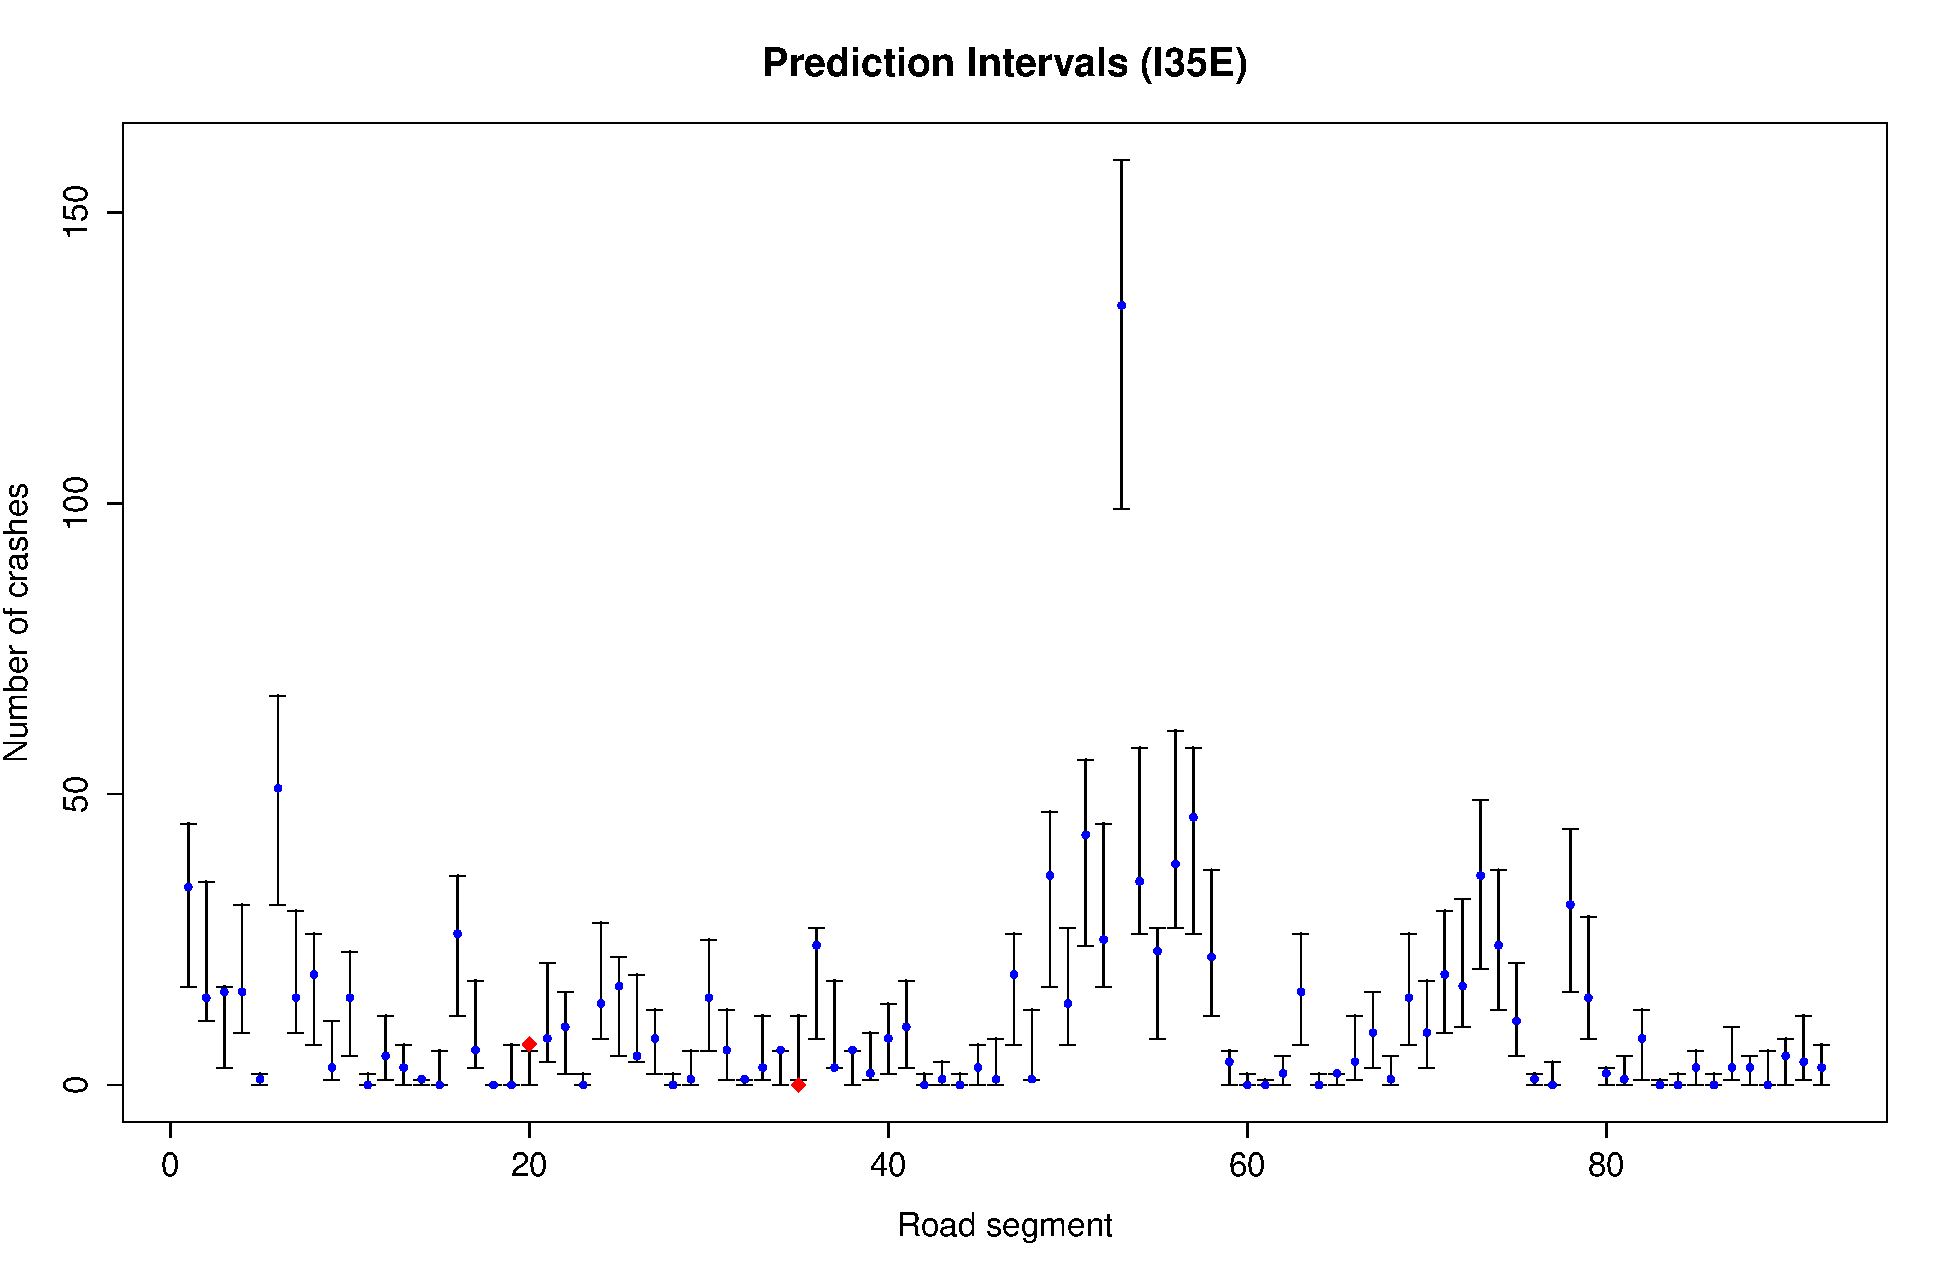
\includegraphics[width=.9\textwidth]{predictive35e.pdf}
\caption{Posterior predictive intervals: blue dots indicate the observed number of crashes fell within a 95\% interval, while red dots indicate the observed crashes did not fall within the interval.}
\label{predictive}
\end{figure}


\section{Results}
The quantity $\mu_s=\exp\{\vec{x}_s'\vec{\beta} + \phi_s\}$ denotes the relative risk (relative to the expected number of crashes $E_s$ from \eqref{Es}) for each road segment where $\mu_s >1$ indicate regions of elevated risk. Figure \ref{relrisk} displays 95\% central credible intervals for each $\mu_s$.  Segments in red correspond to locations where the posterior probability that $\mu_s > 1$ is greater than 0.95 whereas segments in blue correspond to those regions where the posterior probability of $\mu_s < 1$ is greater than 0.95.  In this context, segments in red can be viewed as road segments that pose a high risk to travelers while blue segments are those that are safer than expected. On the I35, three percent of segments (7) have relative risks of over two. I35E has, in general, a much higher relative risk rate than I35. Ten percent (10) road segments have relative risks of higher than 2  and over one-third of segments on the I35E have relative risks over one.  The road segments with a high relative risk should have high priority for systemic improvement.  
\begin{figure}[tb] 
\centering
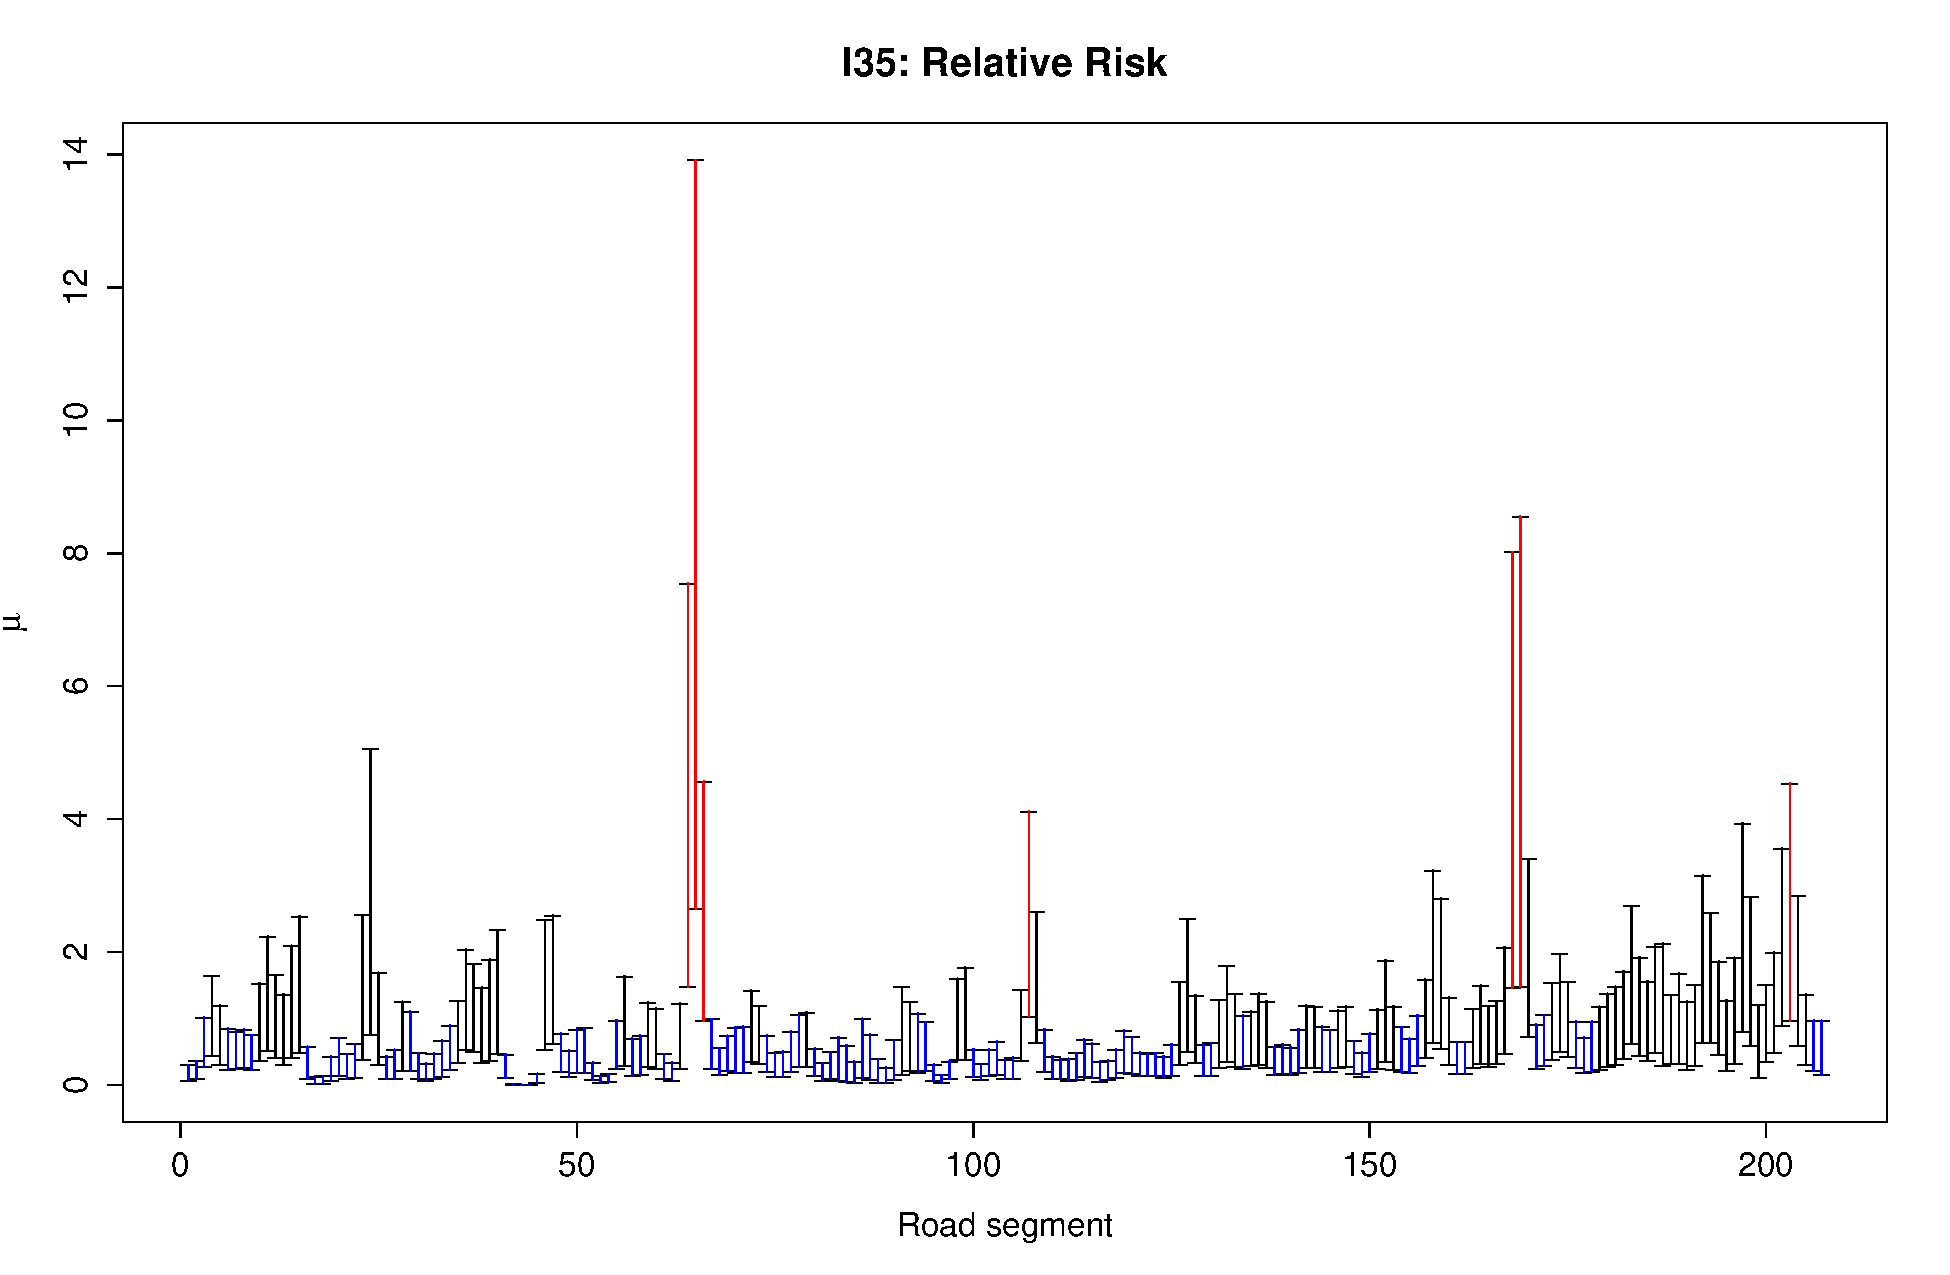
\includegraphics[width=.9\textwidth]{relrisk.pdf}
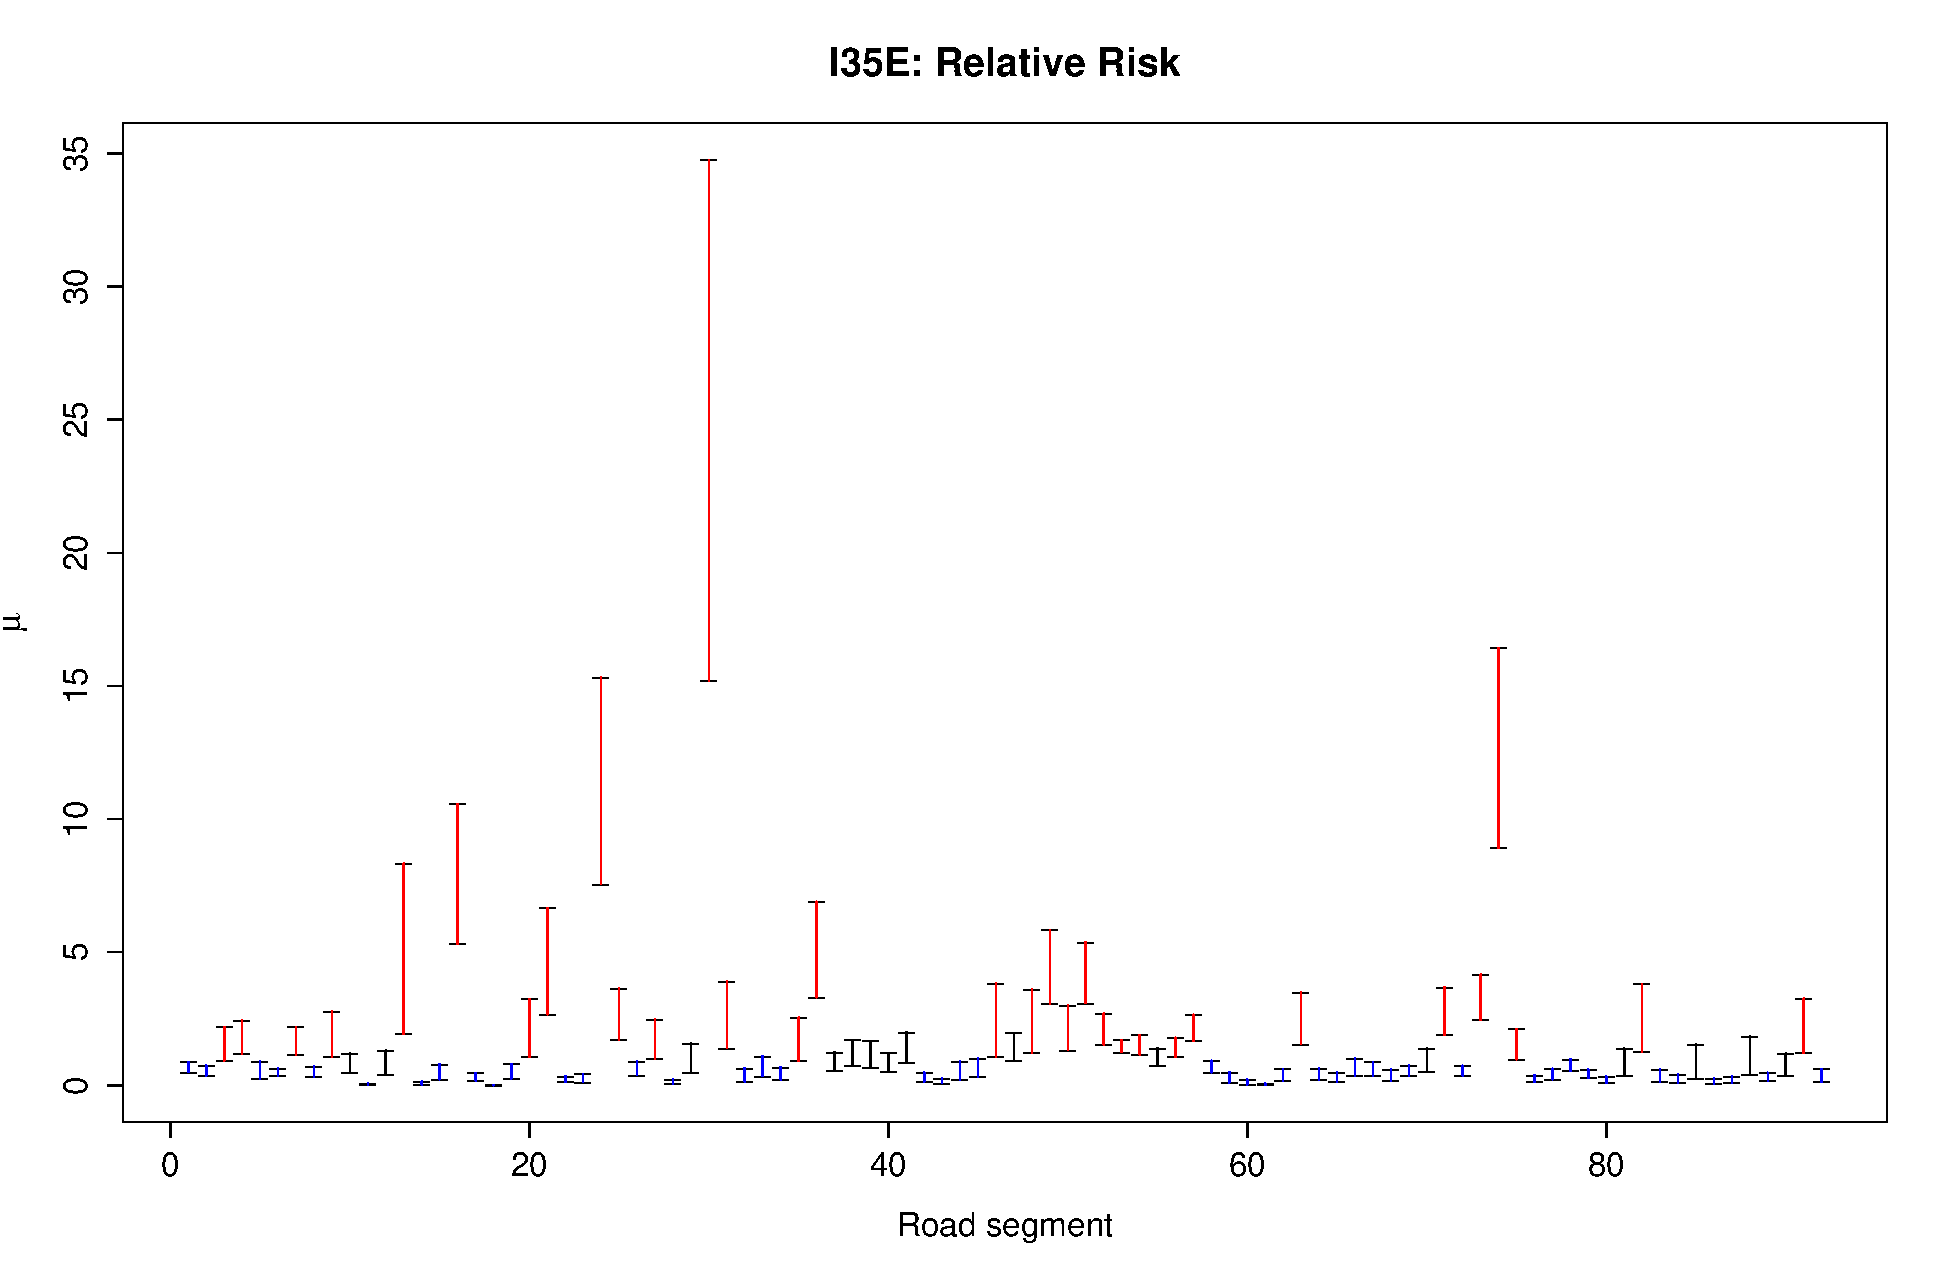
\includegraphics[width=.9\textwidth]{i35erelrisk.pdf}
\caption{95\% credible intervals for the relative risks. Red lines indicate that 95\% of  draws are above 1 (indicating an increased risk of an accident) and blue lines indicate that 95\% of draws are below 1 (indicating a decreased risk of an accident). }
\label{relrisk}
\end{figure}


As described in Chapter 3, the $\beta$ coefficients give the increase (or decrease) in the relative risks associated with an increase in each road characteristic. For example, if $\beta_p > 0$ then  increases in road characteristic $x_p$ are associated with increased relative risk of accidents. Table \ref{beta} shows the central 95\% credible intervals for the intercept and each of the 9 road characteristics. Interestingly, road characteristics have different effects on two highways. On the I35, four covariates are above zero: poor pavement conditions, small and/or variable median width, road width, and right shoulder width. Small median width in particular stands out as having a large, positive association with increased risk of accidents. Hence, safer roads typically have large, constant, median widths, wide left shoulders and fewer lanes. On the I35E, the majority of road characteristics are below zero. Only left shoulder type and road width have a $P(\beta_i>0)$ of over .5 with probabilities of .85 and .66 respectively.
\begin{table}[tb] \centering 
  \caption{95\% central credible intervals for the coefficient of each road characteristic included in this analysis for I35 and I35E.} 
  \label{beta} 
\begin{tabular}{@{\extracolsep{5pt}} lcccccc} 
\hline \hline & \multicolumn{3}{c}{I35} & \multicolumn{3}{c}{I35E} \\ 
 & 2.5\% & 97.5\% & Mean & 2.5\% & 97.5\% & Mean \\ 
\hline \\[-1.8ex] 
Intercept & $$-$1.690$ & $$-$0.460$ & $$-$1.038$ & $2.602$ & $4.081$ & $3.380$ \\ 
Median width $<$ 30ft & $0.557$ & $1.053$ & $0.828$ & $$-$0.869$ & $0.095$ & $$-$0.398$ \\ 
Median width varies & $0.222$ & $0.492$ & $0.366$ & $$-$0.940$ & $$-$0.201$ & $$-$0.567$ \\ 
No median barrier & $$-$0.241$ & $0.255$ & $0.007$ & $$-$1.126$ & $$-$0.294$ & $$-$0.753$ \\ 
Left shoulder width (ft) & $$-$0.120$ & $$-$0.005$ & $$-$0.064$ & $$-$0.175$ & $$-$0.029$ & $$-$0.105$ \\ 
Left shoulder type other & $$-$0.182$ & $0.051$ & $$-$0.069$  & $$-$0.115$ & $0.362$ & $0.114$ \\ 
Road surface width (ft) & $$-$0.012$ & $0.050$ & $0.021$ & $$-$0.045$ & $0.054$ & $0.010$ \\ 
Right shoulder width & $0.078$ & $0.219$ & $0.150$ & $$-$0.139$ & $0.023$ & $$-$0.052$ \\ 
Number of lanes & $$-$0.466$ & $0.015$ & $$-$0.235$ & $$-$0.357$ & $0.229$ & $$-$0.089$ \\ 
Lane width (ft) & $$-$0.006$ & $0.010$ & $0.002$ & $$-$0.199$ & $$-$0.050$ & $$-$0.129$ \\ 
\hline \hline
\end{tabular} 

%\begin{tabular}{@{\extracolsep{5pt}} lccc} 
%\\[-1.8ex]\hline 
%\hline \\[-1.8ex] 
%\textbf{I35E} & 2.5\% & 97.5\% & Mean \\ 
%\hline \\[-1.8ex] 
%Intercept  & $2.602$ & $4.081$ & $3.380$ \\ 
%Median width $<$ 30ft & $$-$0.869$ & $0.095$ & $$-$0.398$ \\ 
%Median width varies & $$-$0.940$ & $$-$0.201$ & $$-$0.567$ \\ 
%No median barrier & $$-$1.126$ & $$-$0.294$ & $$-$0.753$ \\ 
%Left shoulder width (ft) & $$-$0.175$ & $$-$0.029$ & $$-$0.105$ \\ 
%Left shoulder type other & $$-$0.115$ & $0.362$ & $0.114$ \\ 
%Road surface width (ft) & $$-$0.045$ & $0.054$ & $0.010$ \\ 
%Right shoulder width & $$-$0.139$ & $0.023$ & $$-$0.052$ \\ 
%Number of lanes & $$-$0.357$ & $0.229$ & $$-$0.089$ \\ 
%Lane width (ft) & $$-$0.199$ & $$-$0.050$ & $$-$0.129$ \\ 
%\hline \\[-1.8ex] 
%\end{tabular}

\end{table} 

The covariates in the model do not a constitute a complete description of each road segment. For this reason the model in Chapter 3 included spatial random effects. Figure \ref{spatial} includes 95\% credible intervals for the spatial effects on each road segment.  Intuitively, segments with a high (low) spatial random effect correspond to areas where unobserved covariates may be increasing (decreasing) the relative risk.

\begin{figure}[h]
\centering
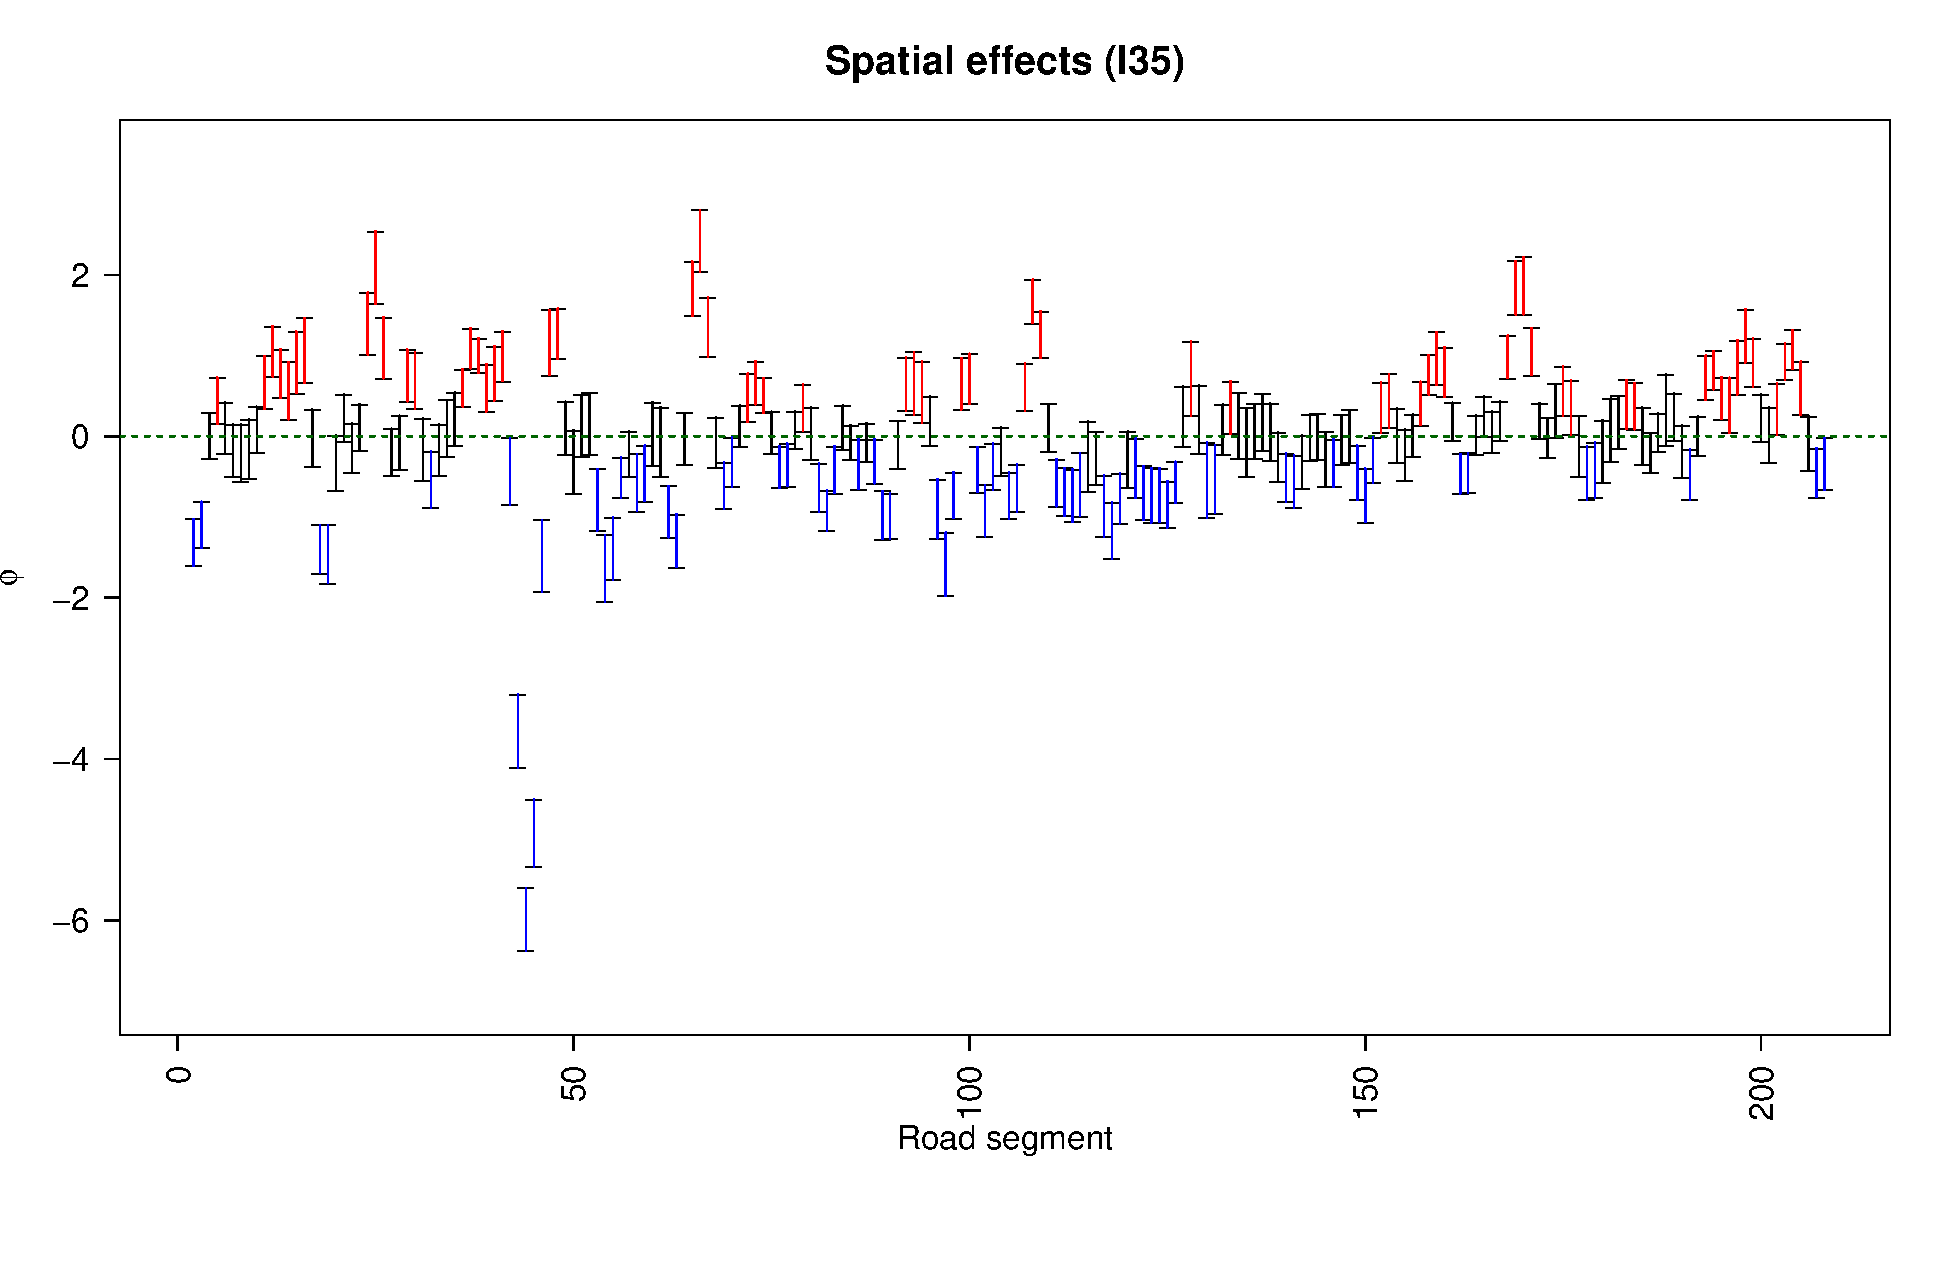
\includegraphics[width=.90\textwidth]{35spatial.pdf}
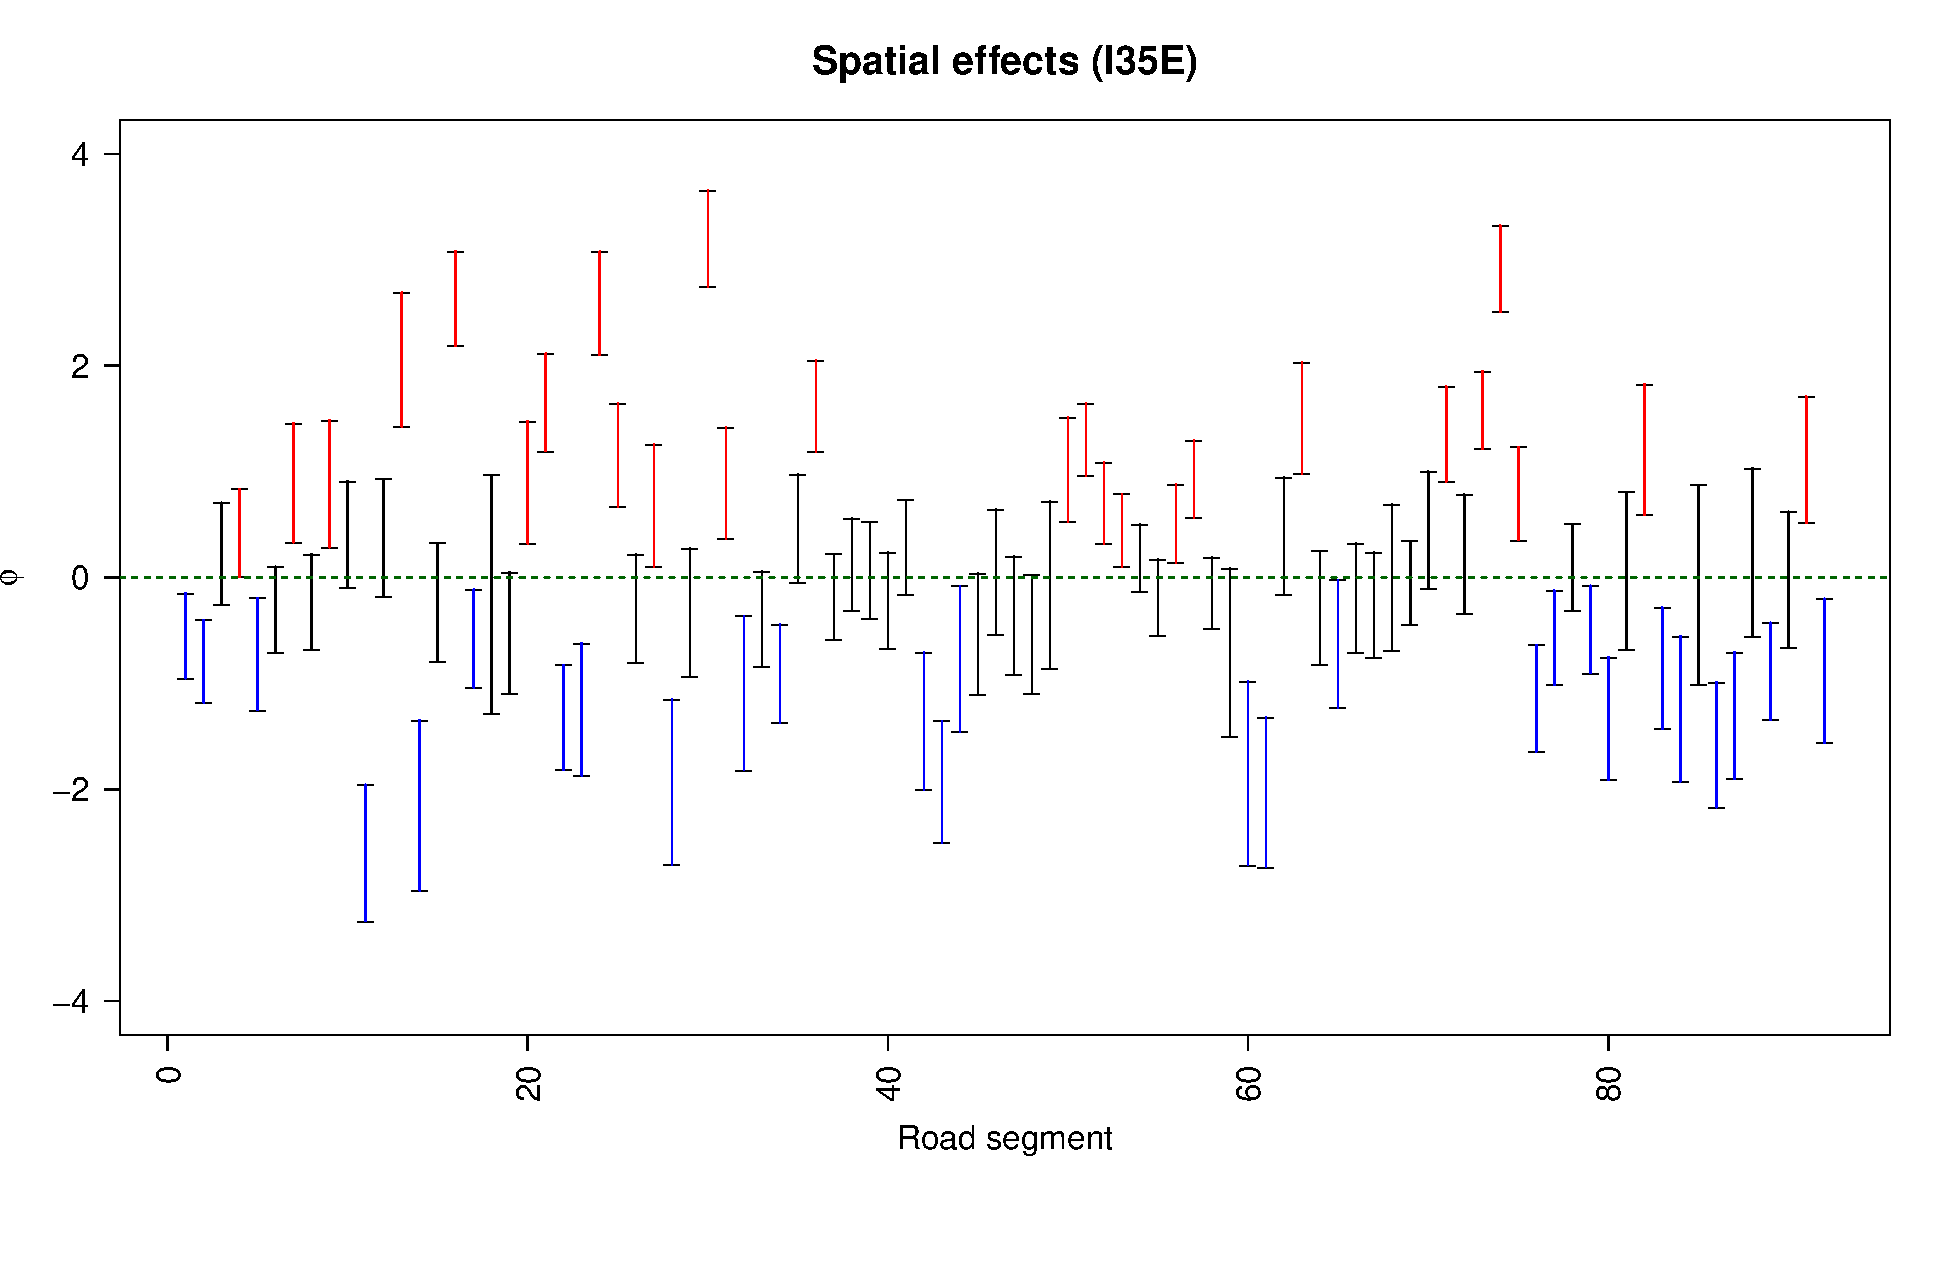
\includegraphics[width=.90\textwidth]{35espatial.pdf}
\caption{95\% credible intervals for the spatial effects. Blue lines indicate the intervals fall below zero while red lines indicate intervals are above zero. }
\label{spatial}
\end{figure}

From Figure \ref{spatial}, notice that segments 180-200 on the I35 (between mile markers 250 and 256) correspond to large spatial random effects. Hence,  these road segments have a higher relative crash rate than we would expect given the observed covariates. Segments 180-200 are associated with freeway segments in the Duluth-Superior metropolitan area. We hypothesize that potential reasons why crash rates are higher in Duluth include not only unobserved characteristics of the road such as high road curvature and steep grades but also  socio-economic variables such as a higher than average number of bars per capita.  However, additional socioeconomic data would be required to verify such claims.


